\documentclass[tikz]{standalone}
\usepackage{graphicx} % Required for inserting images
\usepackage{tikz}
\usetikzlibrary{shadows}
\usepackage{xcolor}
\usetikzlibrary{backgrounds}
\usetikzlibrary {shapes.geometric}

\usetikzlibrary {arrows.meta,automata,positioning,fit,calc}

\definecolor{ProcessStepBackground}{HTML}{FFFAF0}
\definecolor{IntermediateStateColour}{HTML}{949698}

\tikzstyle{NetworkLevel} =[draw,trapezium,trapezium stretches body,trapezium left angle=100, trapezium right angle=100]
\tikzstyle{InfinitesimalNode}=[circle,draw=none,inner sep=0pt,minimum size=0pt]
\tikzstyle{ProcessStepNode} =[draw,fill=ProcessStepBackground,rounded corners,text width=2 cm,align=center]
\tikzstyle{IdleState} =[fill=yellow,rounded corners]
\tikzstyle{OutputState} =[fill=red,rounded corners]
\tikzstyle{InputState} =[fill=green,rounded corners]
\tikzstyle{IntermediateState} =[fill=IntermediateStateColour,rounded corners]
\tikzstyle{Source} =[fill=ProcessStepBackground,shape border rotate=90,aspect=0.1,draw]
\tikzstyle{Sink} =[fill=ProcessStepBackground,shape border rotate=90,aspect=0.1,draw]
\tikzstyle{SourceOrSink} =[fill=ProcessStepBackground,cylinder, shape border rotate=90,aspect=0.1,draw,text width=2 cm,align=center]
\tikzset{
diagonal fill/.style 2 args={fill=#2, path picture={
\fill[#1, sharp corners] (path picture bounding box.south west) -|
                         (path picture bounding box.north east) -- cycle;}},
reversed diagonal fill/.style 2 args={fill=#2, path picture={
\fill[#1, sharp corners] (path picture bounding box.north west) |- 
                         (path picture bounding box.south east) -- cycle;}}
}

\tikzstyle{InputAndOutputState} =[diagonal fill={red}{green},rounded corners, drop shadow,draw ]

\begin{document}
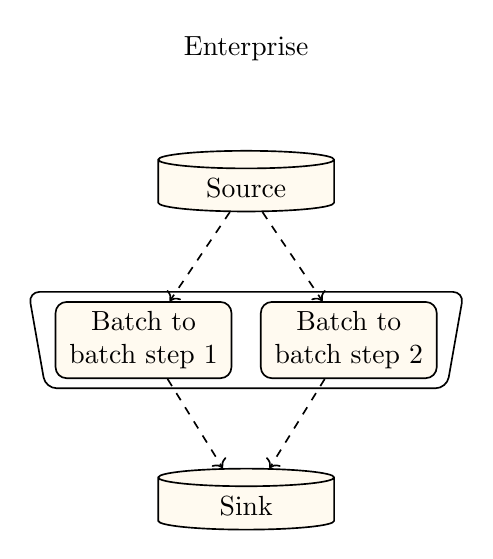
\begin{tikzpicture}[->,auto,node distance=1cm,on grid,semithick]
\node[SourceOrSink](Sink){Sink};
\matrix [column sep=10,row sep=10,draw, rounded corners,nodes={rectangle, anchor=center},NetworkLevel,above= of Sink.north](207433cf-bf92-45da-a5ec-bb94143164c4){
\node[ProcessStepNode](Batch-to-batch-step-1){Batch to batch step 1};&
\node[ProcessStepNode](Batch-to-batch-step-2){Batch to batch step 2};\\
};
\node[SourceOrSink,above= of 207433cf-bf92-45da-a5ec-bb94143164c4.north](Source){Source};
\node[,above= of Source.north](TitleNode){Enterprise};
\draw[dashed] (Source) -> (Batch-to-batch-step-1);
\draw[dashed] (Batch-to-batch-step-1) -> (Sink);
\draw[dashed] (Source) -> (Batch-to-batch-step-2);
\draw[dashed] (Batch-to-batch-step-2) -> (Sink);
\end{tikzpicture}
\end{document}
